\clearpage
\subsection{Literal} % (fold)
\label{sec:program-creation-literal}

A Literal is a whole, or part of, an \nameref{sub:expression} where the value is entered directly into the code.

\begin{figure}[h]
   \centering
   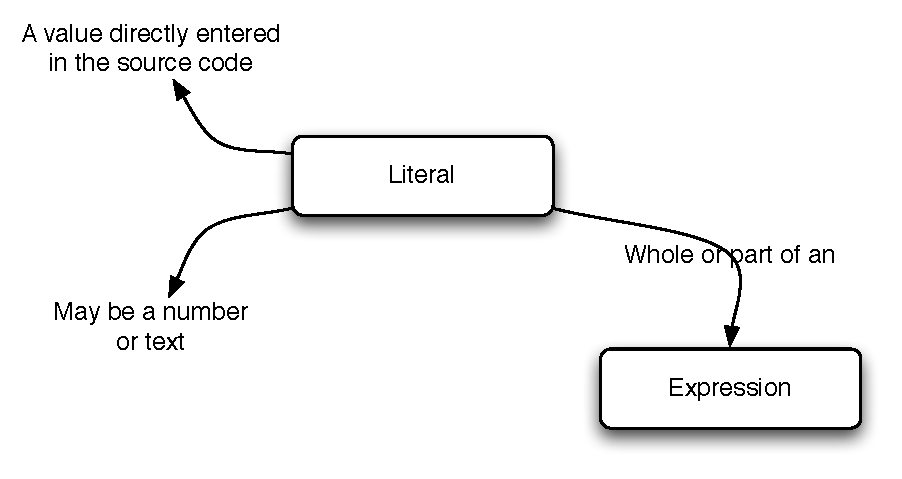
\includegraphics[width=0.8\textwidth]{./topics/program-creation/diagrams/Literal} 
   \caption[Literal Concept Diagram]{Concepts related to Literals.}
   \label{fig:program-creation-literal}
\end{figure}


\mynote{
\begin{itemize}
  \item Figure \ref{fig:program-creation-literal} shows the concepts relate to Literals.
  \item A Literal is a value entered directly into the program's source code.
  \item The value of a Literal can be a number or text.
  \item A Literal can be part or all of an \nameref{sub:expression}.
  \item These values are \emph{hard coded} into the program.
\end{itemize}
}

% section program (end)